\documentclass[onecolumn, draftclsnofoot,10pt, compsoc]{IEEEtran}
\usepackage{graphicx}
\graphicspath{ {images/} }
\usepackage{url}
\usepackage[colorlinks = true,
            linkcolor = blue,
            urlcolor  = blue,
            citecolor = blue,
            anchorcolor = blue]{hyperref}
\usepackage{setspace}
\usepackage{listings}

\usepackage{geometry}
\geometry{textheight=9.5in, textwidth=7in}
\bibliographystyle{IEEEtran}

% 1. Fill in these details
\def \CapstoneTeamName{		COALFO}
\def \CapstoneTeamNumber{		28}
\def \GroupMemberOne{			Kenny Thompson}
\def \GroupMemberTwo{			Bryce Egley}
\def \CapstoneProjectName{		Coal and Open-pit surface mining impacts on American Lands Follow-On (COAL-FO) - Turning spectro-imagery into usable data}
\def \CapstoneSponsorCompany{	NASA JPL}
\def \CapstoneSponsorPerson{		Lewis John Mcgibbney}

% 2. Uncomment the appropriate line below so that the document type works
\def \DocType{	%Problem Statement
				%Requirements Document
				%Technology Review
				%Design Document
				Progress Report
				}

\newcommand{\NameSigPair}[1]{\par
\makebox[2.75in][r]{#1} \hfil 	\makebox[3.25in]{\makebox[2.25in]{\hrulefill} \hfill		\makebox[.75in]{\hrulefill}}
\par\vspace{-12pt} \textit{\tiny\noindent
\makebox[2.75in]{} \hfil		\makebox[3.25in]{\makebox[2.25in][r]{Signature} \hfill	\makebox[.75in][r]{Date}}}}
% 3. If the document is not to be signed, uncomment the RENEWcommand below
\renewcommand{\NameSigPair}[1]{#1}

%%%%%%%%%%%%%%%%%%%%%%%%%%%%%%%%%%%%%%%
\begin{document}
\begin{titlepage}
    \pagenumbering{gobble}
    \begin{singlespace}
    	%\includegraphics[height=4cm]{coe_v_spot1}
        \hfill
        % 4. If you have a logo, use this includegraphics command to put it on the coversheet.
        %\includegraphics[height=4cm]{CompanyLogo}
        \par\vspace{.2in}
        \centering
        \scshape{
            \huge CS Capstone \DocType \par
            {\large\today}\par
            \vspace{.5in}
            \textbf{\Huge\CapstoneProjectName}\par
            \vfill
            {\large Prepared for}\par
            \Huge \CapstoneSponsorCompany\par
            \vspace{5pt}
            {\Large\NameSigPair{\CapstoneSponsorPerson}\par}
            {\large Prepared by }\par
            Group\CapstoneTeamNumber\par
            % 5. comment out the line below this one if you do not wish to name your team
            \CapstoneTeamName\par
            \vspace{5pt}
            {\Large
                \NameSigPair{\GroupMemberOne}\par
                \NameSigPair{\GroupMemberTwo}\par
            }
            \vspace{20pt}
        }
        \begin{abstract}
        % 6. Fill in your abstract
        	Coal and Open-pit surface mining impacts on American Lands Follow-On (COAL-FO) is the successor 				project to the 2016-2017 COAL project. COAL initially aimed to deliver a suite of algorithms to identify, classify, characterize, and quantify (by reporting a number of key metrics) the direct and indirect impacts of mining operations and related destructive surface mining activities across the continental U.S (and further afield). COAL successfully delivered a Python library for processing hyperspectral imagery from remote sensing devices such as the Airborne Visible/InfraRed Imaging Spectrometer (AVIRIS) and a Science Data System for running COAL pipelines. COAL-FO will utilize recent funding obtained from a recently awarded NSF-funded XSEDE high performance computing (HPC) grant to further improve, validate and document COAL algorithms, execution runtime performance and geospatial output results.[1]
        \end{abstract}
    \end{singlespace}
\end{titlepage}
\newpage
\pagenumbering{arabic}
\tableofcontents
% 7. uncomment this (if applicable). Consider adding a page break.
%\listoffigures
%\listoftables
\clearpage

% 8. now you write!
\section{Briefly recap the project purposes and goals}

\noindent This project will take existing algorithms, improve them, and test the ability to work on other systems, as well as improving the overall 'toolkit' of pycoal for the end user. The \href{https://capstone-coal.github.io/team}{COAL-FO} is a continuation of a previous project completed in the 2016-2017 capstone class. The \href{https://capstone-coal.github.io/}{COAL} project was a stable python toolkit providing examples, tests, packages, stable release and stable API that identified, classified, and quantified the effects of open-pit mining on the surrounding environment. Which also included \href{https://github.com/capstone-coal/coal-sds}{COAL-SDS} (Coal Science Data System). Our project will aim at improving the existing algorithms and general functionality as well as enabling the toolkit to work with more spectral libraries. \newline

\section{Describes where you are currently on the project}
This quarter we updated pycoal to work with USGS Spectral Library Version 7. We did this by creating a conversion class in mineral to convert the entire spectral library into a suitable format for saving it as convolved envi files. We then ran classifications using the new spectral library and observed how we could now identify more spectra through our mineral classifications. \newline \newline
We also got into communication with people at USGS about how we would go about creating the convolved library files for USGS Spectral Library 7. The people at USGS recommended we use a software called PRISM. While this software did the job it is not open source, so we would prefer not to use and have our own conversion function since pycoal is meant to be an open source project. \newline \newline
After creating the conversion function for USGS Spectral Library Version 7, we then created unit tests to test the functionality of the conversion function.  We also updated the CLI to accept both USGS Spectral Library Version 6 and USGS Spectral Library Version 7 since we didn’t want to drop support for either of them.

\section{Describe what you have left to do}

We still have to make an update to the website informing users of pycoal how to run the conversion function and how to use the PRISM option of conversion sent to us by USGS. This conversion class can easily be applied to accommodate other spectral libraries such as ECOStress and ECOSIS spectral libraries, which were the requirements we had for this project on pycoal. \newline \newline
We also plan on making instructions to show users how to modify the conversion class so it will work with ECOStress and ECOSIS Spectral Libraries and get them into convolved envi format.

\section{Describe any problems that have impeded your progress, with any solutions you have}

Upgrading to USGS Spectral Library Version 7 was a very long issue that ended up being a lot harder that we had originally anticipated. At first we thought the issue may take a week or two but it ended up taking about 8 weeks when it actually came down to getting the entire spectral library into the correct envi file format, creating unit tests for the conversion function and then running several mineral classifications on the new convolved spectral envi library files. 

\section{Includes particularly interesting pieces of code (if coding is involved)}

USGS Spectral Library Version 7 conversion code \newline
\begin{lstlisting}
class FullSpectralLibrary7Convert:
    def __init__(self):
        """
            This class method converts the entire `USGS Spectral Library Version 7
            <https://speclab.cr.usgs.gov/spectral-lib.html>`_ library into
            its convolved envi format
            
            Args:
            none
            """
        pass

    @classmethod
    def convert(cls, library_filename=""):
        """
            This class method converts the entire `USGS Spectral Library Version 7
            <https://speclab.cr.usgs.gov/spectral-lib.html>`_ library into
            its convolved envi format
            
            Spectral Library Version 7 can be downloaded `here <https://speclab.cr.usgs.gov/spectral-lib.html>`_
            
            Args:
            library_filename (str): path to USGS Spectral Library Version 7 directory
            """
        if not library_filename:
            raise ValueError("Must provide path for USGS Spectral Library Version 7.")
        
        #This will take all the necessary .txt files for spectra in USGS
        #Spectral Library Version 7 and put them in a new directory called
        #"usgs_splib07_modified" in the examples directory
        directory = 'usgs_splib07_modified'
        if not os.path.exists(directory):
            os.makedirs(directory)

        for root, dir, files in os.walk(library_filename + "/ASCIIdata"):
            dir[:] = [d for d in dir]
            for items in fnmatch.filter(files, "*.txt"):
                if "Bandpass" not in items:
                    if "errorbars" not in items:
                        if "Wave" not in items:
                            if "SpectraValues" not in items:
                                shutil.copy2(os.path.join(root,items), directory)

        #This will take the .txt files for Spectra in USGS Spectral Version 7 and
        #convert their format to match that of ASTER .spectrum.txt files for spectra
        # create a new mineral aster conversion instance
        spectral_aster = SpectalToAsterFileFormat()
        #List to check for duplicates
        spectra_list = []
        # Convert all files
        files = os.listdir(directory +'/')
        for x in range(0, len(files)):
            name = directory+'/' + files[x]
            #Get name
            input_file = open(name,'r')
            spectra_line = input_file.readline()
            spectra_cut = spectra_line[23:]
            spectra_name = spectra_cut[:-14]
            #Remove first and last char in case extra spaces are added
            spectra_first_space = spectra_name[1:]
            spectra_last_space = spectra_first_space[:-1]
            
            #Check if Spectra is unique
            set_spectra = set(spectra_list)
            if not any(spectra_name in s for s in set_spectra):
                if not any(spectra_last_space in a for a in set_spectra):
                    spectral_aster.convert(name)
                    spectra_list.append(spectra_name)

        set_spectra = set(spectra_list)
        print(set_spectra)

        #This will generate three files s07av95a_envi.hdr, s07av95a_envi.hdr.sli,splib.db and dataSplib07.db
        #For a library in `ASTER Spectral Library Version 2.0 <https://asterweb.jpl.nasa.gov/>`_ format
        data_dir = "dataSplib07.db"
        header_name = "s07_AV95_envi"

        # create a new mineral aster conversion instance
        spectral_envi = AsterConversion()
        # Generate .sli and .hdr
        spectral_envi.convert(directory,data_dir,header_name)
\end{lstlisting}
Code for unit tests of USGS Spectral Library 7 conversion function
\newline
\begin{lstlisting}
# test files for FullSpectralLibrary7Convert conversion test
_test_SpectralConversion_data = 'usgs_splib07'
_test_SpectralConversion_dir = 'usgs_splib07_modified'
_test_SpectralConversion_db = 'dataSplib07.db'
_test_SpectralConversion_envi = 's07_AV95_envi'

# tear down FullSpectralLibrary7Convert conversion test by deleting test files
def _test_spectral_conversion_teardown():
    _remove_files([_test_SpectralConversion_db,
                   _test_SpectralConversion_dir])

# verify that a small subset of the USGS Spectral Library 7 is converted to ENVI format
@with_setup(None, _test_spectral_conversion_teardown)
def test_spectral_conversion():
    data, dir, db, envi = _test_SpectralConversion_data, _test_SpectralConversion_dir, _test_SpectralConversion_db, _test_SpectralConversion_envi
    spectral_conversion = mineral.FullSpectralLibrary7Convert()
    spectral_conversion.convert(library_filename=data)
    spectral7 = spectral.open_image(envi+'.hdr')
    assert isinstance(spectral7, spectral.io.envi.SpectralLibrary)
\end{lstlisting}

\section{Includes images of your project -- screen shots, photos, whatever is appropriate}

USGS Spectral Library version 6 classification image
\newline
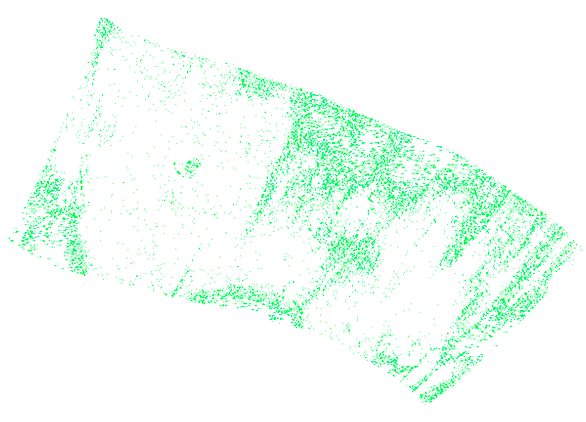
\includegraphics{S06_1}
USGS Spectral Library version 7 classification image \newline
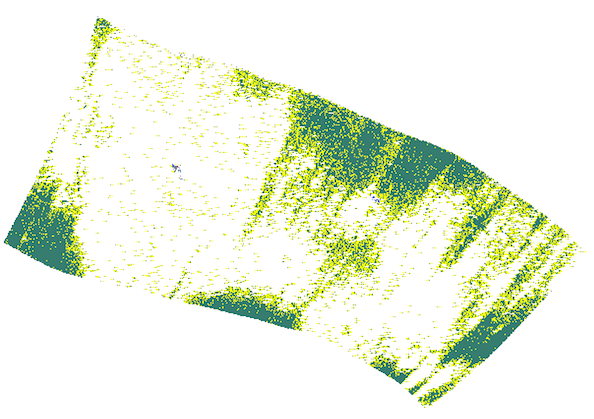
\includegraphics{SO7_1}
USGS Spectral Library version 6 classification of San Juan Coal Mine \newline
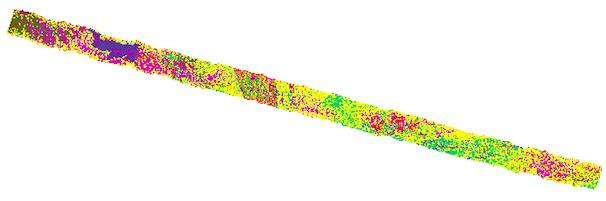
\includegraphics{SO6_2}
USGS Spectral Library version 7 classification of San Juan Coal Mine \newline
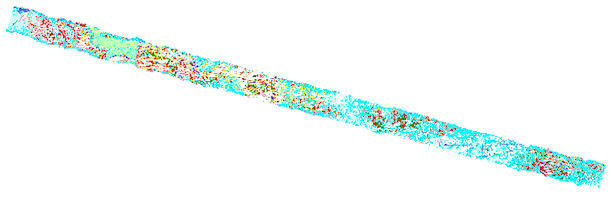
\includegraphics{S07_2}

\begin{thebibliography}{9}
\bibitem{1} ”CS461 - CS Senior Capstone”, Eecs.oregonstate.edu, 2017. [Online]. Available: \url{http://eecs.oregonstate.edu/capstone/cs/capstone.cgi?project=320} [Accessed: 22- Nov- 2017]

\bibitem{2} ”USGS.gov — Science for a changing world”, Usgs.gov, 2017. [Online]. Available: \url{https://www.usgs.gov/} [Accessed: 22- Nov- 2017]

\bibitem{3} ]”AVIRIS - Airborne Visible / Infrared Imaging Spectrometer”, Aviris.jpl.nasa.gov, 2017. [Online]. Available:
\url{https://aviris.jpl.nasa.gov/} [Accessed: 22- Nov- 2017].

\bibitem{4} ”XSEDE User Portal — Globus User Guide”, Portal.xsede.org, 2017. [Online]. Available: \url{https://portal.xsede.org/software/globus} [Accessed: 22- Nov- 2017].

\bibitem{5} ”C++”, En.wikipedia.org, 2017. [Online]. Available:
\url{https://en.wikipedia.org/wiki/C} [Accessed: 22- Nov- 2017].

\bibitem{6} "MySQL", En.wikipedia.org, 2017. [Online]. Available: \url{https://en.wikipedia.org/wiki/MySQL} [Accessed: 22- Nov- 2017].

\bibitem{7} "XSEDE, Extreme Science and Engineering Discovery Environment", www.xsede.org, 2017. [Online]. Available: \url{https://www.xsede.org/} [Accessed: 22- Nov- 2017].

\bibitem{8} "AVIRIS, Airborne Visible/Infrared Imaging Spectrometer", aviris.jpl.nasa.gov, 2017. [Online]. Available: \url{https://aviris.jpl.nasa.gov/} [Accessed: 22- Nov- 2017].

\bibitem{9} "AVIRIS-NG, airborne Visible/Infrared Imaging Spectrometer Next Generation", aviris-ng.jpl.nasa.gov, 2017. [Online]. Available: \url{https://aviris-ng.jpl.nasa.gov/}[Accessed: 22- Nov- 2017].

\bibitem{10} "COAL, Coal and Open-pit surface mining impacts on American Lands", capstone-coal.github.io, 2017. [Online]. Available: \url{https://capstone-coal.github.io/} [Accessed: 22- Nov- 2017].

\bibitem{11} "HPC, High Performance Computing", en.wikipedia.org, 2017. [Online]. Available: \url{https://en.wikipedia.org/wiki/Supercomputer} [Accessed: 22- Nov- 2017].

\bibitem{12} "Query Language", en.wikipedia.org, 2017. [Online]. Available: \url{https://en.wikipedia.org/wiki/Query_language} [Accessed: 22- Nov- 2017].

\bibitem{13} "Enterprise Module Service", hpccsystems.com, 2017. [Online]. Available: \url{https://hpccsystems.com/enterprise-services/modules/esp} [Accessed: 22- Nov- 2017].

\bibitem{14} "HPCC High Performance Computing Cluster", hpccsystems.com, 2017. [Online]. Available: \url{https://hpccsystems.com/enterprise-services/modules/esp} [Accessed: 22- Nov- 2017].

\bibitem{15} "OSU Unix HPC Cluster", cosine.oregonstate.edu, 2017. [Online]. Available \url{http://cosine.oregonstate.edu/unix-hpc-cluster} [Accessed: 22- Nov- 2017].

\bibitem{16} "MIT License", en.wikipedia.org, 2017. [Online]. Available: \url{https://en.wikipedia.org/wiki/MIT_License} [Accessed: 29- Nov- 2017].

\bibitem{17} "Apache License Version 2.0", www.apache.org, 2017. [Online]. Available \url{https://www.apache.org/licenses/LICENSE-2.0} [Accessed: 29- Nov- 2017].

\bibitem{18} "GNU General Public License, version 2", www.gnu.org, 2017. [Online]. Available \url{https://www.gnu.org/licenses/old-licenses/gpl-2.0.en.html} [Accessed: 29- Nov- 2017].

\bibitem{19} "Top Open Source Licenses",www.blackducksoftware.com, 2017.[Online]. Available \url{https://www.blackducksoftware.com/top-open-source-licenses} [Accessed: 29- Nov- 2017].
\end{thebibliography}

\end{document}

